\documentclass{article}
\usepackage[T1]{fontenc}
\usepackage[utf8]{inputenc}
\usepackage[frenchb]{babel}
\usepackage{graphicx}
\usepackage{subcaption}
\usepackage{geometry}
\usepackage{wrapfig}

\title{Lancer de rayon — Première partie}
\author{Simon \textsc{Chopin} \and Marie-Morgane \textsc{PAUMARD}}
\date{\today}

\begin{document}

\maketitle
\tableofcontents
\begin{abstract}
    Ce rapport décrit une implémentation d'un moteur de \emph{lancer de rayon} 
    qui est une technique de \emph{rendu 3D} caractérisée par le \emph{réalisme}
    de ses résultats. Le moteur a été codé en \emph{C++}, et se limite au rendu
    de \emph{sphères}, l'objectif principal étant un système \emph{extensible}.
    
\end{abstract}

\paragraph{Mots-clef}
lancer de rayon ; raytracing ; raycasting ; C++ ; réflexion ; réfraction ;
backend camera.

\section{Introduction}
\subsection{Présentation}
Le lancer de rayon est une technique de synthèse d’image. Il s’agit de calculer
les trajectoires des rayons lumineux depuis la caméra jusqu’à l’objet, puis de
l’objet jusqu’à la source.
Nous avons traité ce projet selon l'approche de Arthur \textsc{Appel} (1968) :
il n'y a ni réflexion ni réfraction, qui seront ajoutées en seconde partie du
projet.

\subsection{Objectifs}
Ce troisième projet de programmation nous a permis de mettre en pratique nos
acquis en C++.

\subsection{Modèle physique}
On se place dans le cadre de l'optique géométrique : il n'y a pas
d'interférences ou de diffraction. Les sphères sont placées dans le vide : il
n'y a donc pas de diffusion, les ombres seront tranchées. Chaque source est
ponctuelle et monochromatique : la lumière blanche est modélisée par la somme
de sources monochromatiques.

\section{Implémentation de base}
\subsection{Description des fonctionnalités}
Dans un premier temps, nous avons souhaité aller au plus simple. Ainsi, la première version du moteur
n'était capable de gérer qu'une seule source de lumière ponctuelle, et les objets ne pouvaient être que 
des sphères. Seules les sources primaires de luminosités sont prises en compte — pas de réflexion ni de
transparence.

\subsection{Diagramme UML}
La création d'un système complexe de classes peut évidemment être faite directement dans le code, 
mais nous avons préféré utiliser un logiciel de modélisation de diagramme UML, BOUML\footnote{Nous
    avons dû utiliser une vieille version, les dernières moutures étant maintenant sous license
propriétaire}. Cela nous a permis de raisonner plus facilement en termes de relations entre les
classes, et nous a également été d'une aide précieuse pour générer un squelette propre et cohérent
pour les sources, ne nous laissant plus que l'implémentation à écrire.

La figure \ref{UML} représente le diagramme sans les améliorations.

\begin{figure}[hbtp]
    \caption{Diagramme UML du moteur de lancer de rayons}
    \label{UML}
    \begin{center}
        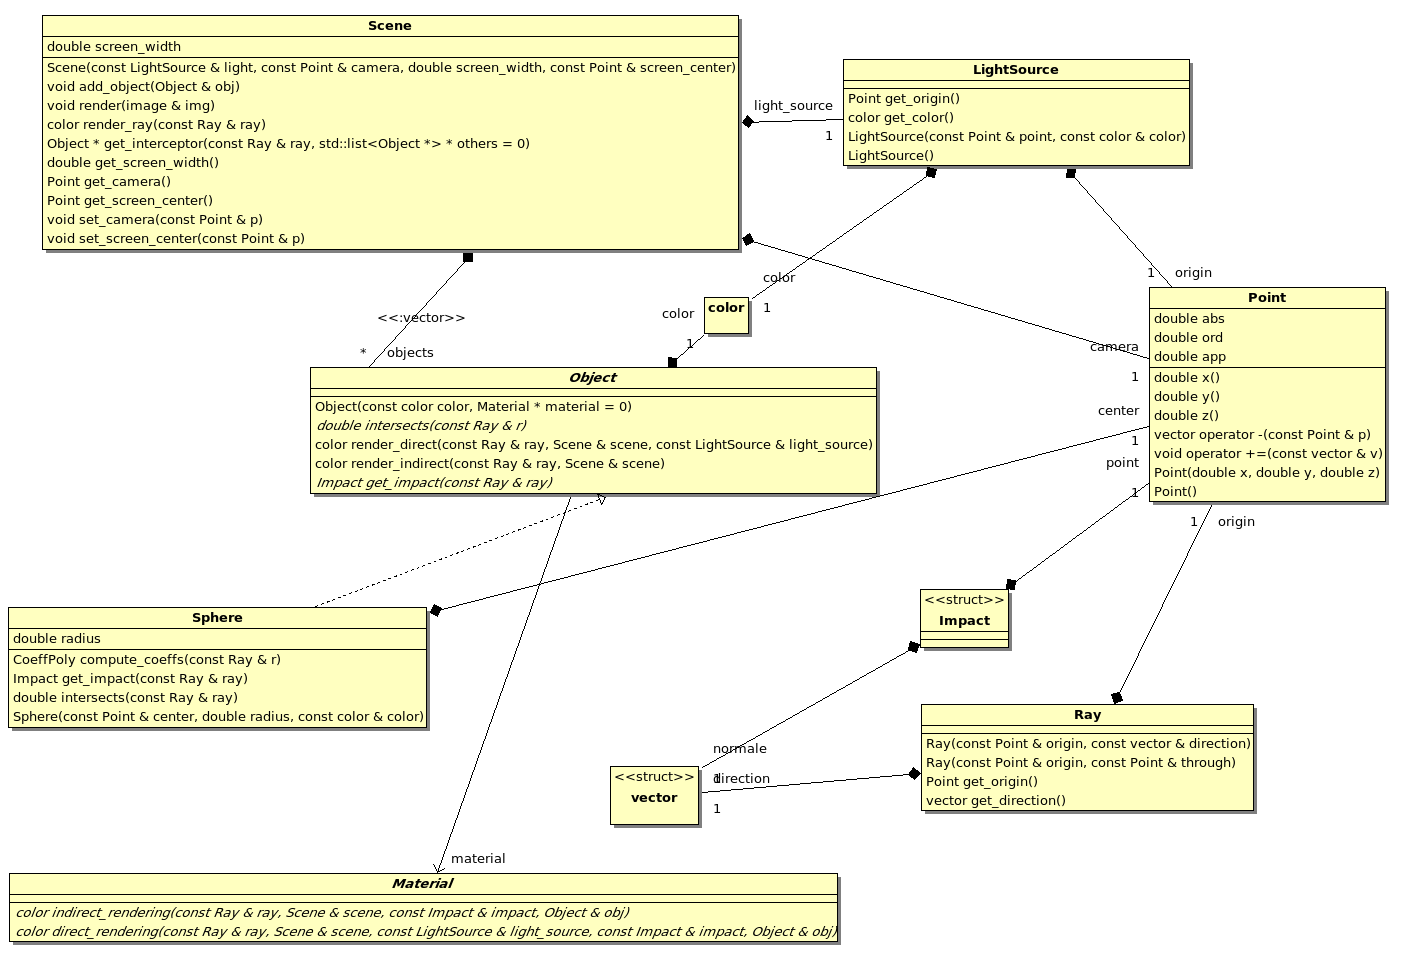
\includegraphics[scale=0.35]{UML}
    \end{center}
\end{figure}

\subsection{Classe \texttt{Scene}}
\begin{wrapfigure}{r}{0.5\textwidth}
    %\vspace{-20pt}
    \caption{Diagramme de la classe Scene}
    \label{scene}
    \begin{center}
    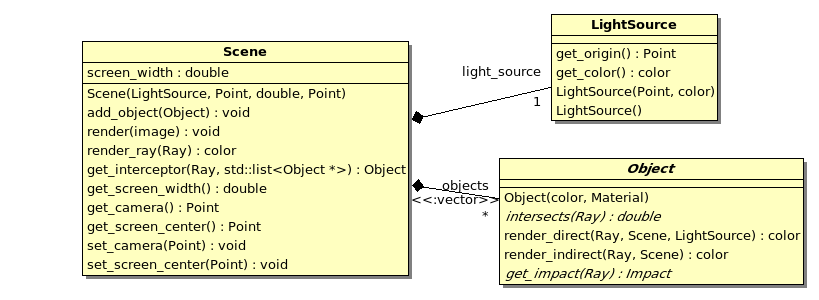
\includegraphics[scale=0.3]{scene.png}
    \end{center}
\end{wrapfigure}

La classe Scene (figure \ref{scene}), et plus spécifiquement sa méthode
\verb,render,, est le point d'entrée du moteur. Nous avons choisi de déclarer la plupart
de ses méthodes comme virtuelles, car la perte de performance nous a paru un faible prix
à payer pour pouvoir bénéficier de la flexibilité que cela, conjugué au découpage fin des
fonctionnalités, apporte au système.

Lors de l'appel à \verb,render,, la première étape est de calculer la position de l'écran
et les distances entre les pixels. Une fois cela fait, un rayon est généré pour chaque
pixel, et la méthode \verb,render_ray, prend le relai.

Cette méthode appelle d'abord \verb,get_interceptor, afin d'obtenir l'objet qui intercepte
le rayon. Si il en existe un, on calcule d'abord la couleur obtenue via les sources secondaires
de lumière — ici, ça sera donc du noir — et la moyenne quadratique\footnote{N'ayant pas la notion
    d'intensité dans nos sources lumineuses, nous nous sommes décidés pour ceci malgré le fait
que ça n'ait aucune base physique} des sources primaires — la seule source de la scène —, et on
"additionne" les deux résultats pour avoir la couleur du pixel.

\subsubsection{Interface de \texttt{get\_interceptor}}
L'interface un peu incongrue de \verb,get_interceptor, est dûe à nos
efforts pour éliminer les artefacts résultant du calcul sur les flottants.

En effet, notamment sur les plans, il arrive que le point calculé à l'interception soit derrière
le plan, ce qui fait que celui-ci est le premier intercepteur du rayon généré. Afin d'éliminer ce
cas-ci, nous avons besoin de la liste des autres intercepteurs si le premier est dans ce cas-là.

\subsection{Classe \texttt{Object}}

La class \verb,Object, est l'abstraction des objets présents sur la scène qui sont susceptibles
d'être illuminés par les sources lumineuses. C'est une classe abstraite, car elle ne possède pas
de notion de volume ou de forme.

À cette fin, toutes les classes implémentant \verb,Object, doivent fournir les méthodes \verb,intercepts,
et \verb,get_impact,, la première donnant la distance entre le point d'origin d'un rayon et son point
d'intersection sur l'objet, et la seconde calculant le point d'intersection et la normale à la surface
de l'objet en ce point.

En plus de cela, un objet peut avoir un pointeur de type \verb,Material,, qui lorsque non-nul permet
de représenter les comportements inhérents au matériau de l'objet au lieu de sa forme. Une des conséquences
de cette approche est qu'une sphère de verre et une sphère d'aluminium auront toutes deux le même type. Une
autre possibilité de ce système est de changer le comportement d'un objet au fil du temps.

\subsection{Utilisation des éléments propres à C++}
\paragraph{Pointeurs}
Bien que notre moteur utilise les pointeurs par nécessité — on ne peut pas utiliser les conteneurs de la
STL avec des références, car il faut des objets qui soient copiables avec un constructeur par défaut —
nous avons préféré ne pas prendre en compte la durée de vie des objets pointés, et préférons laisser à
l'utilisateur le soin de s'assurer de la validité des données fournies, notamment des objets, tout le long
de l'utilisation du moteur.

\paragraph{Sous-classe et implémentation dans le header}
Dans la classe Sphère, il faut à plusieurs endroits calculer des résultats à partir des coefficients d'une
équation du second degré. Pour faciliter la manipulation de ces coefficients, nous avons créé une sous-classe
de Sphere que nous avons souhaité garder privée, car elle fait partie des détails d'implémentation.

Cependant, pour ce faire, nous avons été forcé de définir une fonction dans le header de \verb,Sphere, car
le compilateur refusait de compiler la définition d'une méthode d'une classe privée en dehors de la classe
à laquelle elle appartenait.

\section{Améliorations}
\subsection{Améliorations réalisées}
\subsubsection{Objets non sphériques}
Pour pouvoir observer les ombres portées, nous avons insérés des plans dans
notre rendu. Il s'agit d'une classe similaire à la classe sphère : elle hérite
également de la classe objet.

Sur la figure ci-dessous, on voit deux plans (l'un jaune, l'autre violet) et
trois sphères. Il y a trois sources monochromatiques.

\begin{center}
  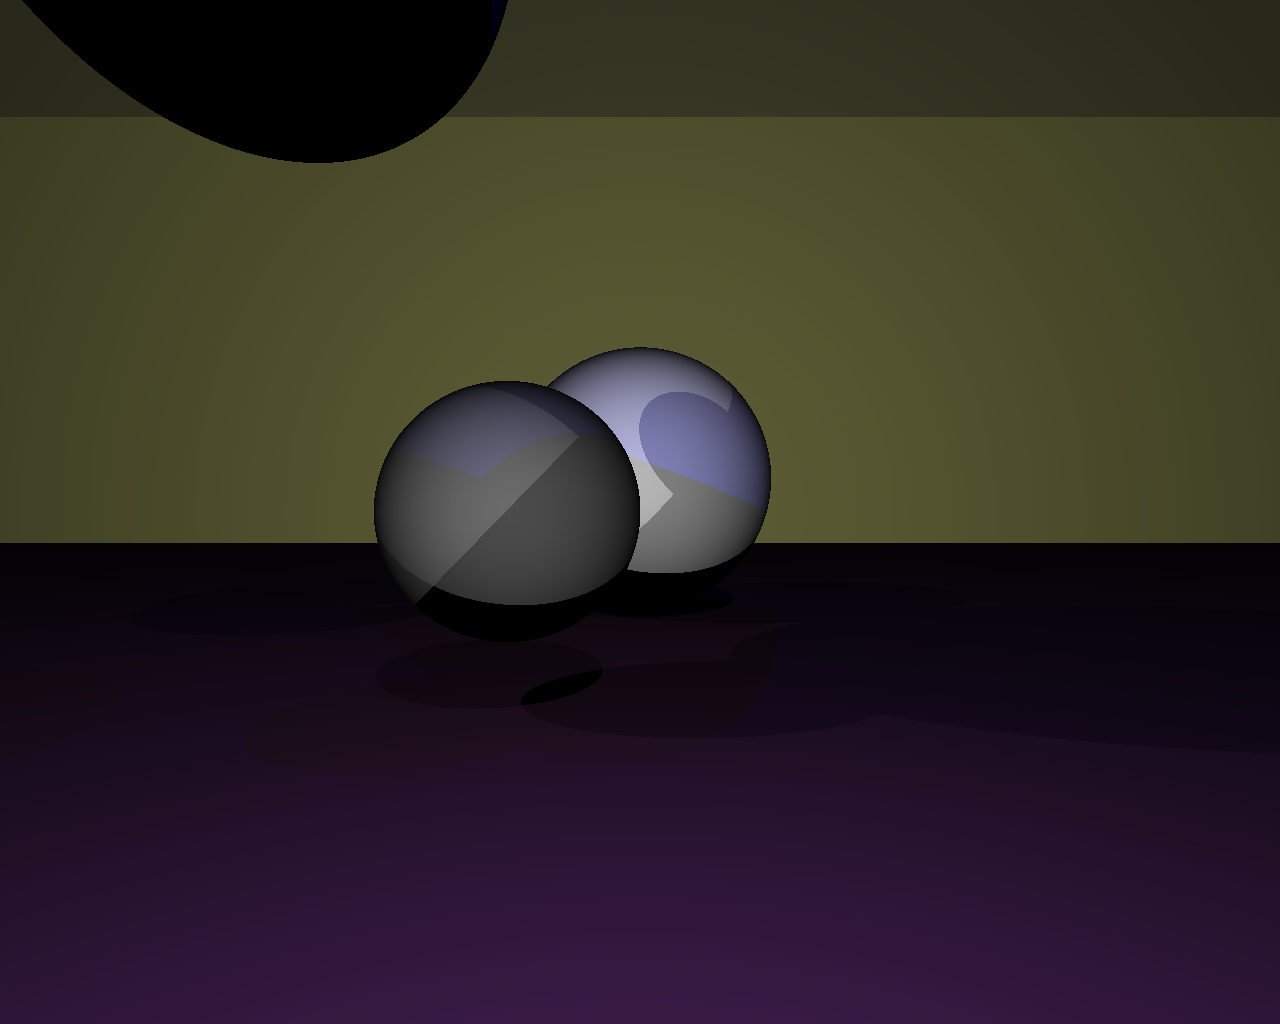
\includegraphics[scale=0.2]{img/screenshot.png}
\end{center}


\subsubsection{Backend camera}

\subsection{Exemples d'améliorations aisément implémentables}
\subsubsection{Gestion des matériaux : la réfraction}
La réfraction est le phénomène de déviation du rayon lumineux qui se produit
lors d’un changement de milieux transparents d’indices différents : sa
trajectoire est modifiée selon sa longueur d'onde.

\begin{center}
  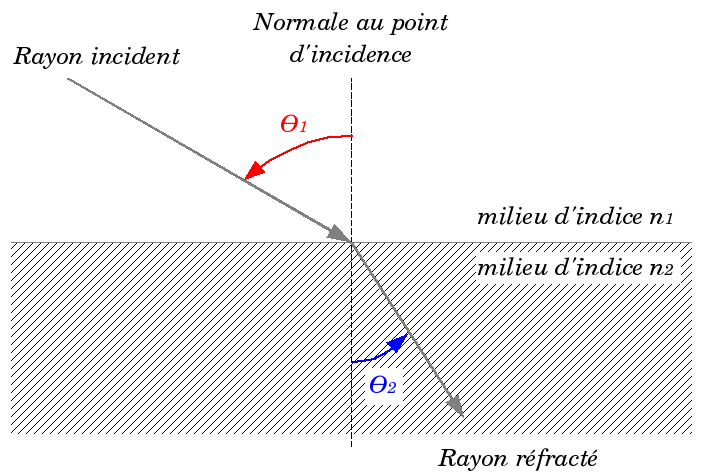
\includegraphics[scale=0.5]{img/refraction.png}
\end{center}

\paragraph{Implémentation}
Dans notre programme, il est aisé de mettre en œubre la réflexion. Pour ce faire
, il suffit de munir la classe objet de l'indice du milieu et d'un coefficient
de transmission.

L'indice du milieu $n$ permet de calculer la déviation du rayon, selon la loi de
\textsc{Snell-Descartes} : $n_i \sin i = n_r \sin r$, où $i$ (respectivement $r$)
est l'angle entre la normale et le rayon incident (respectivement réfléchi). $n$
vaut 1 dans le vide et représente la vitesse du rayon dans le milieu divisée par
la célérité de la lumière.

Le coefficient de transmission $t$ nous permet de calculer l'intensitée lumineuse
transmise par le milieu. Si $t=1$, le milieu se comporte comme le vide ; si $t=0$,
il réagit comme un milieu opaque, ce qui correspond au cas étudié dans cette
première partie du projet. On a : $t=\frac{2n_i}{n_i + n_r}$.

\paragraph{Milieux}
Cette extension permet de se placer dans un milieu autre que le vide. On peut
ainsi imaginer vouloir traiter le milieu comme un objet : il disposerait d'une
couleur et de coefficients de transmission et réflexion. On peut par exemple se
placer dans un gaz très dense, dans lequel les objets lointains ne sont plus que
de vagues formes désaturées.

\subsubsection{Gestion des matériaux : la réflexion}
La réflexion est un phénomène de déviation du rayon lumineux : en arrivant
sur une surface, une partie du rayon est renvoyé.

\begin{center}
  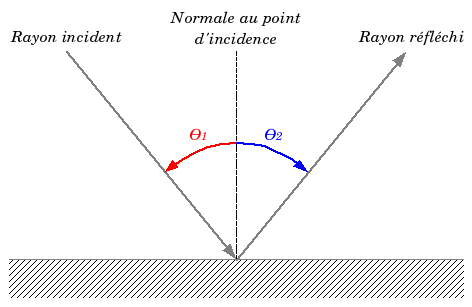
\includegraphics[scale=0.5]{img/reflexion.png}
\end{center}

\paragraph{Implémentation}
Pour implémenter la réflexion, on munit la classe objet de l'indice du milieu et
d'un coefficient de réflexion $r$.

Ce coefficient est obtenu par la loi : $r= \frac{n_i - n_r}{n_i + n_r}$. On a
donc $1+r=t$.

\section{Conclusion}
Le lancer de rayon est un projet intéressant : outre les habituelles réflexions
de conceptions, nous avons du veiller à fournir un code modulable, dans 
l'optique de se voir réutilisé en seconde partie.


\appendix
\section{Bibliographie}

\end{document}
